\chapter{Diseño de la solución, arquitectura y selección tecnológica}
\label{chap:diseno-arquitectura}

\section{Propósito y enfoque arquitectónico}

Este capítulo traduce los requerimientos del capítulo anterior en una arquitectura concreta, organizada en tres repositorios desacoplados que colaboran mediante contratos HTTP explícitos, persistencia, trazabilidad distribuida y revisión profesional obligatoria. La separación entre experiencia de usuario, lógica de producto y procesamiento especializado es estricta por diseño, y el sistema no emite diagnóstico autónomo ni considera aceptada una salida sin revisión humana.

La documentación sigue el modelo de vistas «4+1» de Kruchten [38], que organiza la descripción en cinco vistas complementarias: lógica, de procesos, de desarrollo, física y de escenarios. Cada una atiende las inquietudes de distintos interesados y, en conjunto, permite verificar que la arquitectura satisface los requerimientos sin repetir la misma información desde perspectivas superpuestas.
\begin{figure}[htbp]
\centering
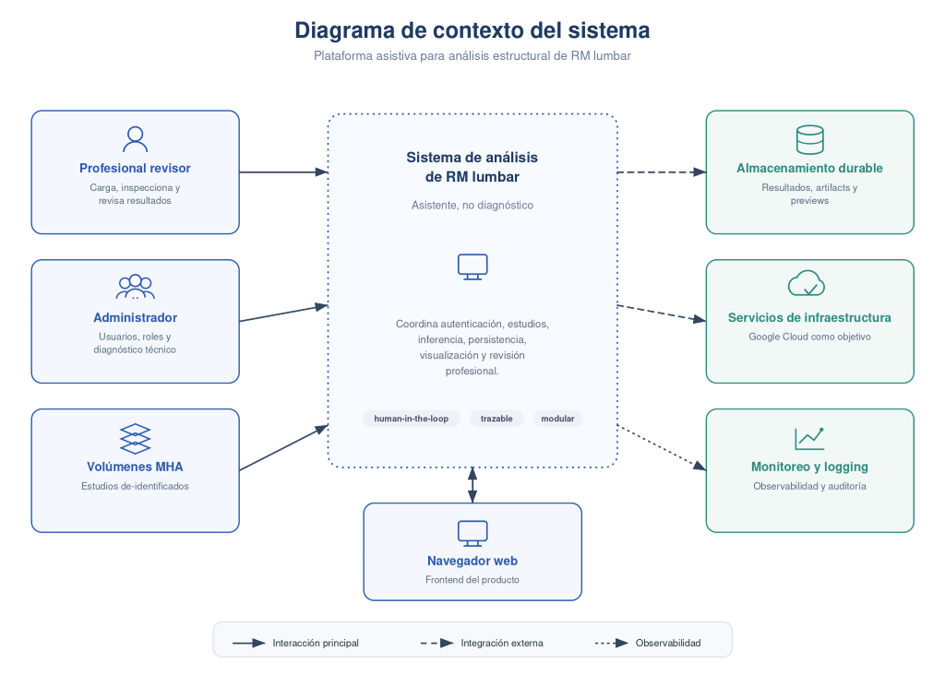
\includegraphics[width=0.92\textwidth]{images/architecture/fig_10_01_contexto_sistema.png}
\caption{Diagrama de contexto del sistema. Fuente: elaboración propia.}
\label{fig:arch-contexto-sistema}
\end{figure}
% STRUCTURE_REVIEW_REQUIRED
% SOURCE_NUMBERING_GAP: 10.2
% DOCX_INLINE_TEXT_AFTER_CAPTION: 10.2 Visión general del flujo
% STRUCTURE_REVIEW_REQUIRED
% SOURCE_NUMBERING_GAP: 10.2
% DOCX_INLINE_TEXT_AFTER_CAPTION: 10.2 Visión general del flujo

El prototipo recibe un estudio de resonancia magnética lumbar que puede incluir el plano sagital, el axial o ambos, y lo recorre en seis etapas. La entrada se carga y se prepara mediante normalización de intensidades y ajuste de formato. La segmentación genera máscaras para las estructuras contempladas en cada plano. El postprocesamiento organiza esas máscaras, las asocia a un nivel anatómico cuando resulta posible y calcula los valores geométricos. La visualización superpone las máscaras sobre la imagen original. La revisión profesional permite aceptar, corregir, observar o descartar cada resultado. La salida editable reúne estructuras, mediciones, unidades, observaciones y estado de revisión, e incluye un preinforme automático revisable.

{\small
\setlength{\LTleft}{0pt}
\setlength{\LTright}{0pt}
\setlength{\tabcolsep}{2pt}
\renewcommand{\arraystretch}{1.18}
\begin{longtable}{>{\raggedright\arraybackslash}p{0.30\textwidth} >{\raggedright\arraybackslash}p{0.62\textwidth}}
\caption{Componentes funcionales del prototipo}\label{tab:arch-componentes-funcionales}\\
\hline
\textbf{Componente} & \textbf{Función principal} \\
\hline
\endfirsthead
\caption[]{Componentes funcionales del prototipo (continuación)}\\
\hline
\textbf{Componente} & \textbf{Función principal} \\
\hline
\endhead
\hline
\endfoot
Entrada y preprocesamiento & Cargar el estudio, preservar su información espacial y prepararlo para la inferencia \\
Segmentación & Delimitar las estructuras anatómicas contempladas en cada plano mediante modelos de aprendizaje profundo \\
Mediciones & Calcular valores geométricos derivados de máscaras visibles y trazables \\
Visualización & Mostrar la imagen original con las máscaras superpuestas y sus resultados asociados \\
Salida editable & Organizar los resultados en una plantilla revisable y un preinforme modificable y no diagnóstico \\
Validación & Comparar máscaras contra anotaciones de referencia y complementar con revisión profesional \\
\hline
\end{longtable}
}

El prototipo opera bajo un enfoque de humano en el circuito: el sistema propone segmentaciones y mediciones, y el profesional conserva la revisión final. Esa condición es necesaria porque las máscaras pueden contener errores, las mediciones requieren contexto y el alcance del proyecto no contempla diagnóstico autónomo. El resultado esperado no se mide únicamente por una métrica de segmentación sino por la coherencia del flujo completo, desde la imagen de entrada hasta la salida revisada. El fundamento conceptual de este enfoque se desarrolla en la sección 7.11 y su implementación en la sección 11.8.
% CROSS_REFERENCE_MAPPING_REQUIRED
% CROSS_REFERENCE_MAPPING_REQUIRED

\section{Decisiones arquitectónicas derivadas de los requerimientos}

Las decisiones principales se derivan de las necesidades de carga, segmentación, visualización, corrección, trazabilidad, seguridad y control profesional. El diseño evita concentrar todas las responsabilidades en una aplicación monolítica y asigna cada capacidad a la capa tecnológica más adecuada.

{\footnotesize
\setlength{\LTleft}{0pt}
\setlength{\LTright}{0pt}
\setlength{\tabcolsep}{2pt}
\renewcommand{\arraystretch}{1.18}
\phantomsection\label{tab:arch-decisiones-requerimientos}
\begin{longtable}{>{\raggedright\arraybackslash}p{0.24\textwidth} >{\raggedright\arraybackslash}p{0.32\textwidth} >{\raggedright\arraybackslash}p{0.36\textwidth}}
\hline
\textbf{Requerimiento o necesidad} & \textbf{Implicancia técnica} & \textbf{Respuesta arquitectónica} \\
\hline
\endfirsthead
\hline
\textbf{Requerimiento o necesidad} & \textbf{Implicancia técnica} & \textbf{Respuesta arquitectónica} \\
\hline
\endhead
\hline
\endfoot
Carga de estudios de-identificados & El caso debe conservar identidad, plano y metadata sin almacenar datos personales innecesarios & Backend para registrar el estudio y Frontend para seleccionar los volúmenes. \\
Segmentación sagital y axial & Coexisten modelos con datasets, clases y artifacts diferentes & Registro por modelKey, ejecución por plano y agrupación bajo multiplanarRunId. \\
Revisión profesional & La salida automática no puede considerarse definitiva & Estados pendiente, aceptado, observado y descartado, con notas y auditoría. \\
Trazabilidad & Cada corrida debe poder explicarse y reproducirse & caseId, runId, multiplanarRunId, traceId, modelVersion, artifactHash y modos de inferencia. \\
Reapertura sin AI Module & Los resultados deben permanecer disponibles aunque el motor de IA esté apagado & Persistencia durable de contratos, mediciones y assets servidos por el Backend. \\
Navegación volumétrica & Un archivo MHA contiene múltiples cortes y el usuario debe poder recorrerlos & Catálogo de slices, previews persistidos, índice seleccionado y visor navegable. \\
No diagnóstico autónomo & El sistema debe asistir sin reemplazar el juicio profesional & humanReviewRequired, notClinicalDiagnosis y ausencia de conclusiones clínicas automáticas. \\
Actualización de modelos & Los checkpoints pueden evolucionar y exceder los límites de GitHub & Código en repositorios; artifacts y manifests en storage externo verificable. \\
Despliegue controlado & La infraestructura debe ser reproducible y limitar costos & Contenedores, variables de entorno, servicios separados y arquitectura objetivo en Google Cloud. \\
\hline
\end{longtable}
}

\section{Vista lógica}

La vista lógica describe la estructura funcional del sistema: sus componentes principales, el modelo de datos y las clases del dominio.

\subsection{Arquitectura lógica consolidada}

La arquitectura se organiza en capas desacopladas. El navegador consume el Frontend; el Frontend se comunica exclusivamente con el Backend de producto; el Backend centraliza autenticación, autorización, persistencia, auditoría, serving de assets y comunicación con el AI Module; y el AI Module encapsula la lógica Python, la gestión de modelos, el runtime PyTorch y la orquestación de inferencia.

{\footnotesize
\setlength{\LTleft}{0pt}
\setlength{\LTright}{0pt}
\setlength{\tabcolsep}{2pt}
\renewcommand{\arraystretch}{1.18}
\phantomsection\label{tab:arch-logica-capas}
\begin{longtable}{>{\raggedright\arraybackslash}p{0.18\textwidth} >{\raggedright\arraybackslash}p{0.22\textwidth} >{\raggedright\arraybackslash}p{0.52\textwidth}}
\hline
\textbf{Capa} & \textbf{Tecnología} & \textbf{Responsabilidad principal} \\
\hline
\endfirsthead
\hline
\textbf{Capa} & \textbf{Tecnología} & \textbf{Responsabilidad principal} \\
\hline
\endhead
\hline
\endfoot
Frontend & React, Vite y TypeScript & Autenticación visual, worklist, alta y consulta de estudios, workspace sagital–axial, visor de cortes, revisión, historial y diagnósticos técnicos. \\
Backend & Spring Boot y Java & Seguridad, reglas de negocio, persistencia, auditoría, proxy hacia IA, contratos canónicos, serving de assets y reapertura. \\
AI Module & Python y FastAPI & Registry de modelos, manifests, hashing, preprocesamiento, inferencia, reportes, catálogo volumétrico y generación de previews. \\
Runtime de inferencia & PyTorch & Reconstrucción de arquitecturas, carga de state\_dict, model.eval(), torch.inference\_mode() y predicción. \\
Persistencia & PostgreSQL & Usuarios, roles, estudios, corridas, revisiones, mediciones, artifacts y eventos de auditoría. \\
Storage de modelos y archivos & Storage externo controlado & Checkpoints, manifests, datasets y, en la arquitectura objetivo, volúmenes y assets durables. \\
Entorno experimental & Google Colab, Drive y notebooks & Entrenamiento, evaluación, generación de checkpoints y evidencia reproducible. \\
\hline
\end{longtable}
}

Esta separación permite desplegar, probar y evolucionar cada módulo con su tecnología natural. También reduce el riesgo de que una modificación del modelo obligue a recompilar la interfaz o que la lógica clínica-asistiva quede mezclada con detalles internos de PyTorch.

La Figura~\ref{fig:arch-componentes} muestra la separación entre Frontend, Backend, AI Module, runtime PyTorch, persistencia y almacenamiento de artifacts.

\begin{figure}[htbp]
\centering
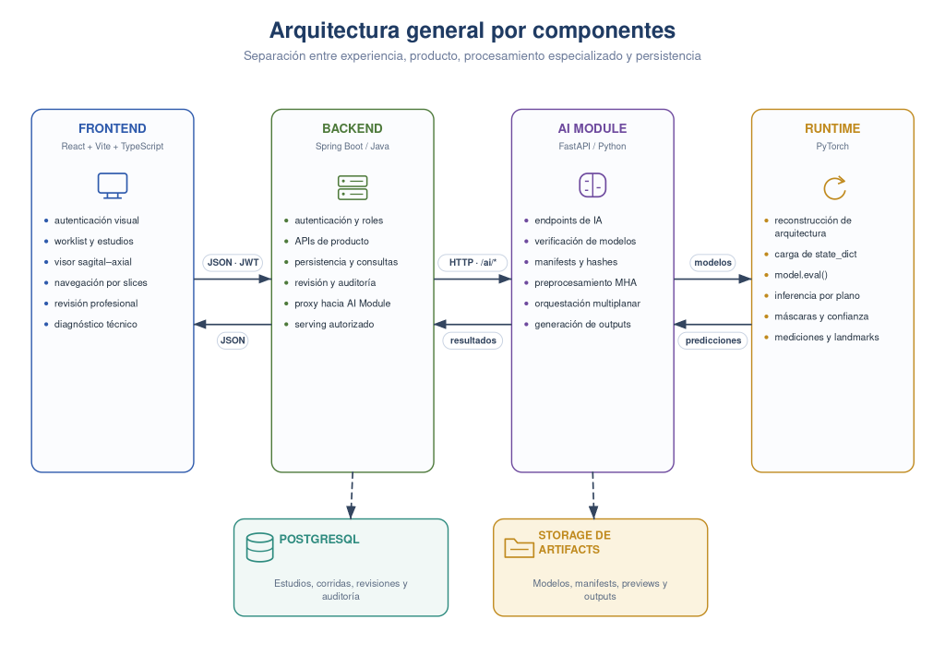
\includegraphics[width=0.92\textwidth]{images/architecture/fig_10_02_componentes.png}
\caption{Arquitectura general por componentes. Fuente: elaboración propia.}
\label{fig:arch-componentes}
\end{figure}
% STRUCTURE_REVIEW_REQUIRED
% DOCX_INLINE_TEXT_AFTER_CAPTION: 10.3.2 Arquitectura volumétrica y visualización de secciones.
% STRUCTURE_REVIEW_REQUIRED
% DOCX_INLINE_TEXT_AFTER_CAPTION: 10.3.2 Arquitectura volumétrica y visualización de secciones.

El sistema ingesta el estudio como DICOM completo, identifica las series y las clasifica por plano y ponderación; los formatos MHA y NIfTI se conservan como compatibilidad técnica. El contrato volumétrico define por serie el plano, el identificador, la cantidad de cortes, el corte seleccionado, el eje, las dimensiones nativa y normalizada, el espaciado y un catálogo en el que cada corte puede asociarse con una vista previa, un indicador de resultados y, cuando corresponda, superposición, puntos de referencia y mediciones.

La responsabilidad se distribuye entre las tres capas: el módulo de inteligencia artificial lee el volumen completo, genera una vista previa por corte y marca los cortes con resultados; el backend persiste volumen, catálogo y vistas previas, y publica los accesos autorizados, de modo que la reapertura funciona con el módulo de inferencia apagado; el frontend presenta el recorrido por cortes con teclado, miniaturas, ajuste visual y navegación desde un resultado hacia su corte de origen.

\begin{figure}[htbp]
\centering
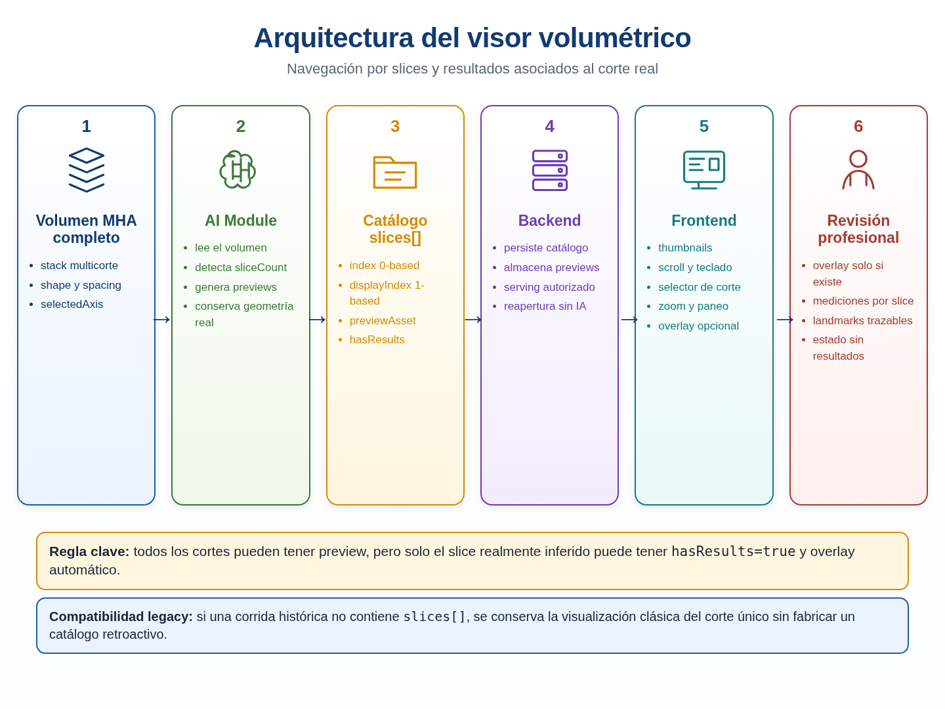
\includegraphics[width=0.92\textwidth]{images/architecture/fig_10_03_visor_volumetrico.png}
\caption{Arquitectura del visor volumétrico. Fuente: elaboración propia.}
\label{fig:arch-visor-volumetrico}
\end{figure}

La superposición automática no se presupone para todos los cortes de todas las series. Se ejecuta segmentación de la serie completa en las modalidades soportadas, y las series no soportadas permanecen disponibles como imagen base, informando que no poseen inferencia automática. El visor no simula una correspondencia espacial entre el plano sagital y el axial cuando la metadata geométrica no permite demostrarla.

\subsection{Modelo de datos}

La persistencia se apoya en un modelo relacional en PostgreSQL organizado alrededor de tres ejes: la identidad y el control de acceso (usuarios, roles), la organización de los estudios (sujeto de-identificado, estudio) y la evidencia de cada análisis (corrida, mediciones, revisiones, assets y catálogo de cortes), complementados con el registro de modelos/artifacts y la auditoría. La Figura~\ref{fig:arch-modelo-datos} presenta el diagrama entidad-relación con sus claves primarias, foráneas y cardinalidades.

El diseño refleja las decisiones descritas en los capítulos anteriores: los datos identificatorios del paciente se almacenan de forma segura (Ley N.º 25.326) y los estudios se vinculan mediante una referencia de sujeto seudonimizada (subject\_ref); cada corrida conserva su linaje técnico (model\_key, artifact\_hash, requested/effective\_inference\_mode y trace\_id); las mediciones y los assets quedan vinculados a la corrida y al corte de origen; y la revisión profesional se registra sin sobrescribir el resultado automático original, preservando la trazabilidad y la auditabilidad.
% CROSS_REFERENCE_MAPPING_REQUIRED

\begin{figure}[htbp]
\centering
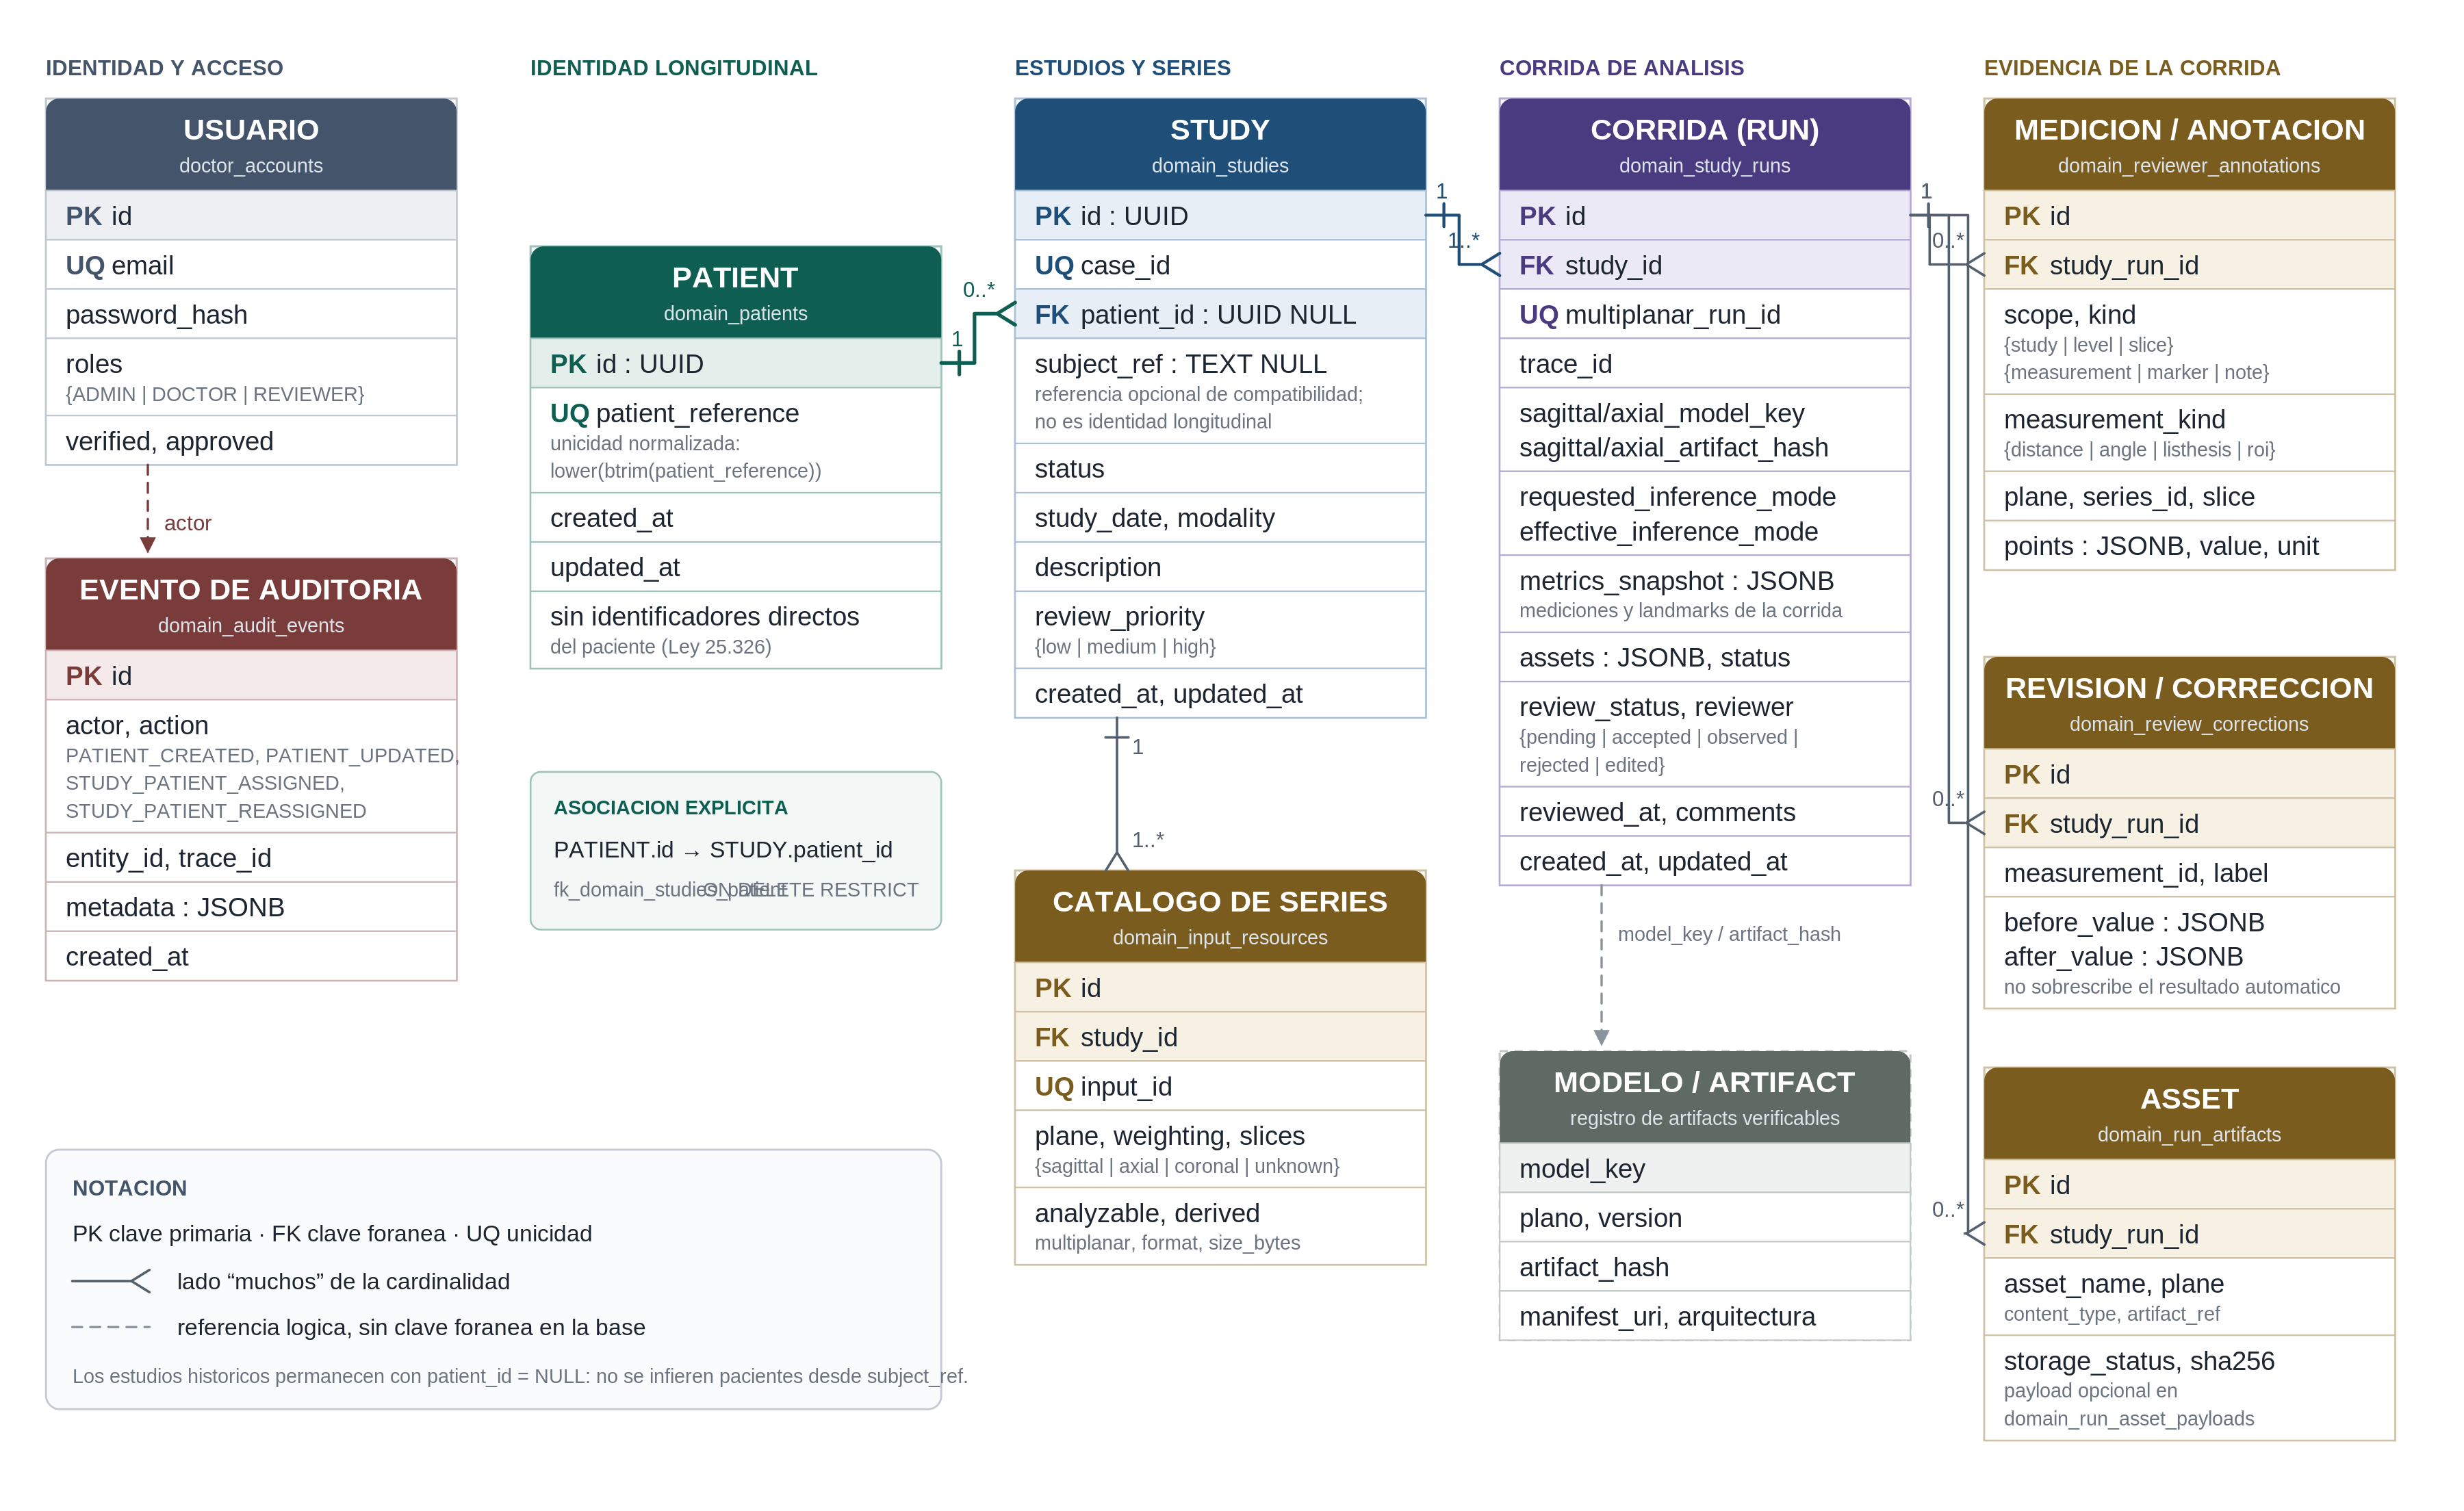
\includegraphics[width=0.92\textwidth]{images/architecture/fig_10_04_modelo_datos.png}
\caption{Modelo de datos relacional (PostgreSQL). Fuente: elaboración propia.}
\label{fig:arch-modelo-datos}
\end{figure}

Entidades principales

{\footnotesize
\setlength{\LTleft}{0pt}
\setlength{\LTright}{0pt}
\setlength{\tabcolsep}{2pt}
\renewcommand{\arraystretch}{1.18}
\phantomsection\label{tab:arch-entidades-principales}
\begin{longtable}{>{\raggedright\arraybackslash}p{0.20\textwidth} >{\raggedright\arraybackslash}p{0.72\textwidth}}
\hline
\textbf{Entidad} & \textbf{Descripción y atributos clave} \\
\hline
\endfirsthead
\hline
\textbf{Entidad} & \textbf{Descripción y atributos clave} \\
\hline
\endhead
\hline
\endfoot
usuario & Cuenta del sistema. Atributos: id (PK), email, password\_hash, estado\_aprobacion, fecha\_registro. \\
rol / usuario\_rol & Roles ADMIN, DOCTOR y REVIEWER, asociados a usuarios mediante una tabla intermedia (relación muchos a muchos). \\
sujeto & Referencia de-identificada del paciente. Atributos: subject\_ref (PK). No almacena datos identificatorios. \\
estudio & Contenedor lógico de un caso. Atributos: study\_id (PK), subject\_ref (FK), creado\_por (FK usuario), fecha, metadata. \\
corrida (run) & Ejecución de análisis por plano. Atributos: run\_id (PK), study\_id (FK), model\_key (FK), plano, multiplanar\_run\_id, artifact\_hash, requested/effective\_inference\_mode, trace\_id, estado. \\
modelo / artifact & Modelo registrado y su artifact verificable. Atributos: model\_key (PK), plano, version, artifact\_hash, manifest\_uri, arquitectura. \\
medicion & Valor geométrico derivado de una máscara. Atributos: id (PK), run\_id (FK), estructura/label, plano, slice\_index, valor, unidad, confidence, estado\_revision. \\
revision & Decisión profesional sobre una corrida. Atributos: id (PK), run\_id (FK), usuario\_id (FK), estado (pendiente/aceptado/observado/rechazado/corregido), comentario, fecha. \\
asset & Archivo derivado servido bajo autorización. Atributos: id (PK), run\_id (FK), rol (input/mask/overlay/…), content\_type, hash, size, url. \\
slice\_catalogo (P10.5) & Catálogo de cortes del volumen para el visor. Atributos: id (PK), run\_id (FK), index, preview\_asset, has\_results. \\
evento\_auditoria & Registro de trazabilidad. Atributos: id (PK), usuario\_id (FK), entidad, accion, trace\_id, timestamp. \\
\hline
\end{longtable}
}

Relaciones principales

\begin{itemize}
  \item Un sujeto agrupa uno o varios estudios; un estudio contiene una o varias corridas.
  \item Cada corrida referencia el modelo/artifact ejecutado y genera múltiples mediciones, assets y entradas del catálogo de cortes.
  \item Una corrida acumula una o varias revisiones profesionales sin eliminar el resultado automático original.
  \item Los usuarios se asocian con roles (muchos a muchos) y quedan registrados como autores de estudios, revisiones y eventos de auditoría.
\end{itemize}

\subsection{Diagrama de clases}

El diagrama de clases presenta las entidades del dominio y los servicios principales, con sus atributos, operaciones y relaciones. La Figura~\ref{fig:arch-clases-dominio} lo resume.
% ORIGINAL_DOCX_REFERENCE: Figura 12.5
% NORMALIZED_TO_DYNAMIC_REFERENCE: YES

\begin{figure}[htbp]
\centering
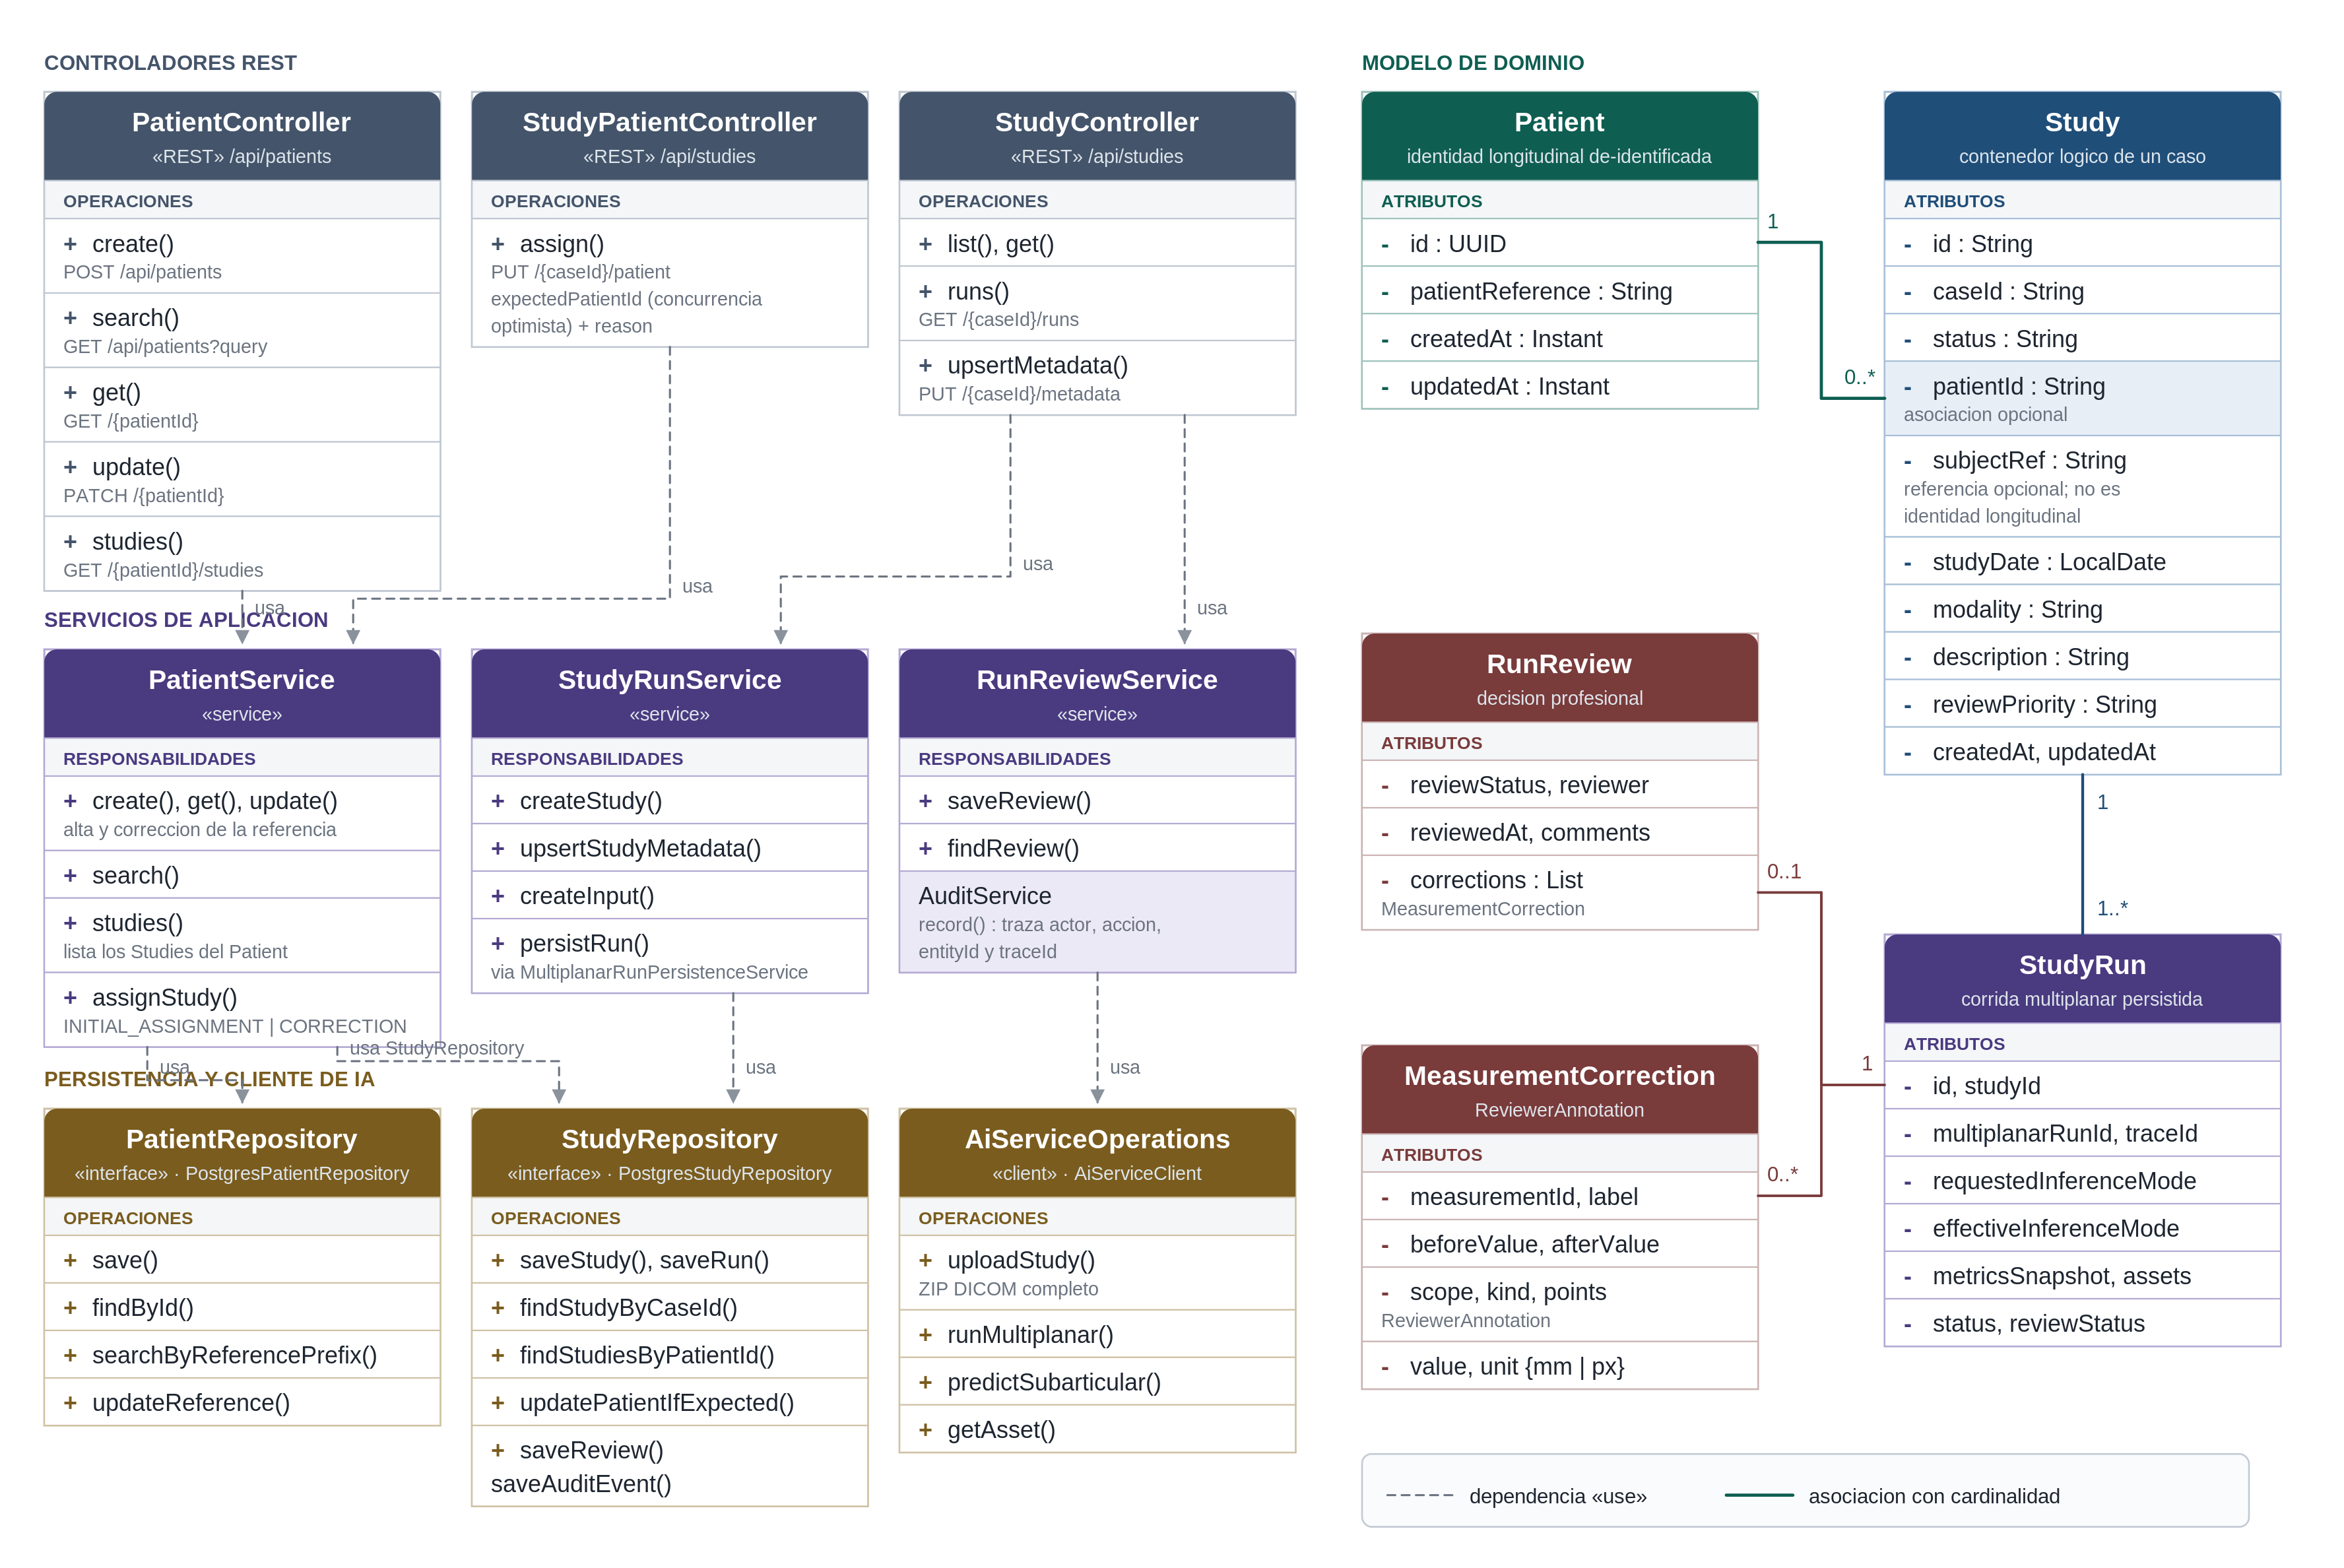
\includegraphics[width=0.72\textwidth]{images/architecture/fig_10_05_clases_dominio.png}
\caption{Diagrama de clases del dominio y servicios. Fuente: elaboración propia.}
\label{fig:arch-clases-dominio}
\end{figure}
% STRUCTURE_REVIEW_REQUIRED
% DOCX_INLINE_TEXT_AFTER_CAPTION: 10.5 Vista de procesos.
% STRUCTURE_REVIEW_REQUIRED
% DOCX_INLINE_TEXT_AFTER_CAPTION: 10.5 Vista de procesos.

La vista de procesos describe el comportamiento en ejecución: la secuencia de una corrida, la persistencia y reapertura, y la comunicación entre servicios.

\section{Vista de procesos}

La vista de procesos describe el comportamiento en ejecución: la secuencia de una corrida, la comunicación entre servicios y el tratamiento de los estados de error.

\subsection{Flujo end-to-end de una corrida}

El flujo principal coincide con el descrito en las secciones 6.1 y 11.5. Desde la perspectiva arquitectónica interesa destacar su trazabilidad extremo a extremo: el estudio ingresa como DICOM completo (ZIP), el Backend identifica y clasifica las series, registra los inputs compatibles (Sagital T1, Sagital T2 y Axial de forma independiente), solicita al AI Module la segmentación de la serie completa y, cuando corresponde, la línea de hallazgos P10.7, y persiste resultados, mediciones y revisión en PostgreSQL. Los formatos MHA/NIfTI se mantienen como compatibilidad técnica, no como flujo principal.
% CROSS_REFERENCE_MAPPING_REQUIRED
% CROSS_REFERENCE_MAPPING_REQUIRED

La arquitectura diferencia requestedInferenceMode de effectiveInferenceMode. Una solicitud real\_baseline solo se informa como efectiva cuando el artifact fue verificado y la ejecución PyTorch finalizó correctamente. Si la ejecución falla, el sistema debe informar error o degradación según la configuración; no debe presentar una respuesta de contrato como inferencia real.

La Figura~\ref{fig:arch-flujo-end-to-end} resume la secuencia completa desde la autenticación y la carga del estudio hasta la persistencia y la revisión profesional.

\begin{figure}[htbp]
\centering
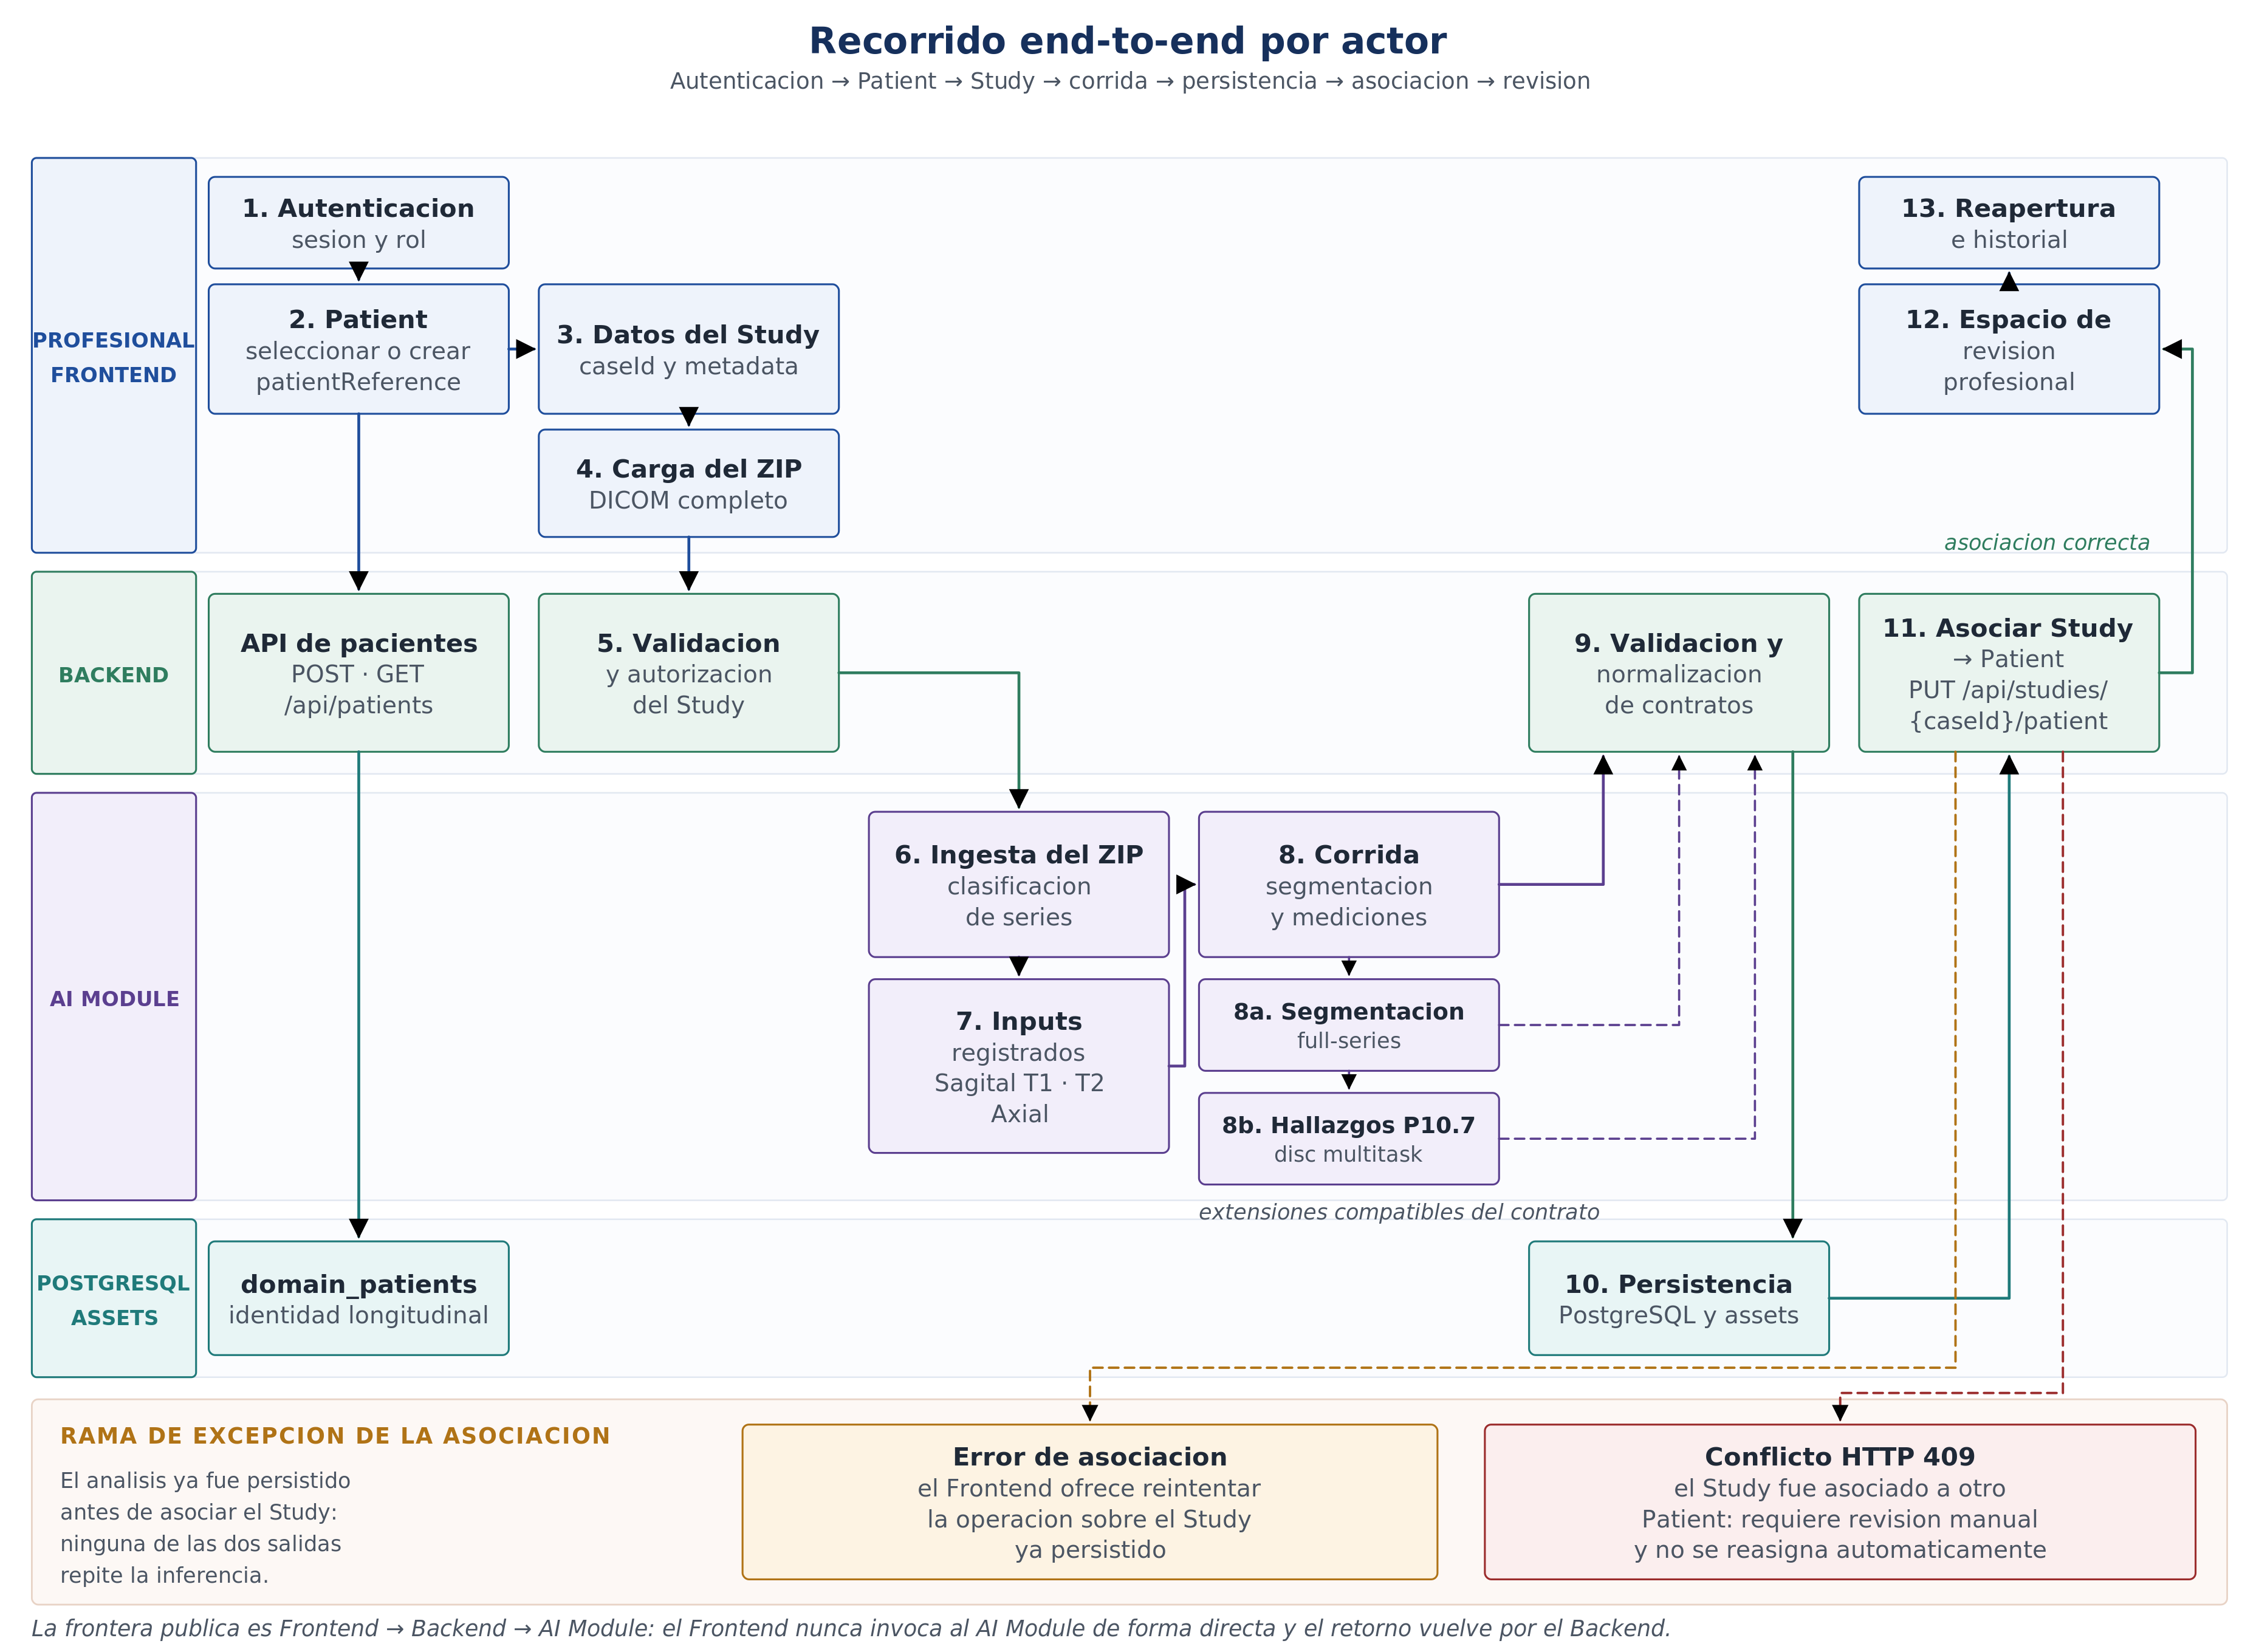
\includegraphics[width=0.92\textwidth]{images/architecture/fig_10_06_flujo_end_to_end.png}
\caption{Flujo de interacción end-to-end. Fuente: elaboración propia.}
\label{fig:arch-flujo-end-to-end}
\end{figure}
% STRUCTURE_REVIEW_REQUIRED
% DOCX_INLINE_TEXT_AFTER_CAPTION: 10.4.2 Persistencia, assets y reapertura.
% STRUCTURE_REVIEW_REQUIRED
% DOCX_INLINE_TEXT_AFTER_CAPTION: 10.4.2 Persistencia, assets y reapertura.

La persistencia se diseña alrededor de la corrida de análisis. Cada estudio conserva contratos canónicos, mediciones, estados de revisión, referencias a assets y datos de auditoría. Los paths internos del AI Module (por ejemplo rutas temporales de contenedor) no forman parte del contrato público.

Los assets se describen mediante nombre, rol, tipo de contenido, hash, tamaño y URL autorizada del Backend. Esta estrategia desacopla el navegador de la ubicación física del archivo y permite mover el almacenamiento sin alterar la interfaz.

La reapertura es un requisito arquitectónico central. Una corrida persistida debe poder visualizarse aunque el AI Module esté detenido. Por esa razón, los previews del stack no se generan bajo demanda desde el motor de IA: deben producirse durante la corrida y persistirse junto con el resto de la evidencia.

\subsection{Arquitectura de red, protocolos y seguridad}

La comunicación entre capas utiliza HTTP(S), contratos JSON versionables y trazabilidad por headers. El navegador se autentica contra el Backend; el Backend propaga el traceId hacia el AI Module; y el AI Module materializa artifacts desde storage externo mediante credenciales administradas fuera del código.

{\footnotesize
\setlength{\LTleft}{0pt}
\setlength{\LTright}{0pt}
\setlength{\tabcolsep}{2pt}
\renewcommand{\arraystretch}{1.18}
\phantomsection\label{tab:arch-red-seguridad}
\begin{longtable}{>{\raggedright\arraybackslash}p{0.16\textwidth} >{\raggedright\arraybackslash}p{0.16\textwidth} >{\raggedright\arraybackslash}p{0.24\textwidth} >{\raggedright\arraybackslash}p{0.36\textwidth}}
\hline
\textbf{Origen} & \textbf{Destino} & \textbf{Mecanismo} & \textbf{Propósito} \\
\hline
\endfirsthead
\hline
\textbf{Origen} & \textbf{Destino} & \textbf{Mecanismo} & \textbf{Propósito} \\
\hline
\endhead
\hline
\endfoot
Navegador & Frontend & HTTPS & Acceso a la interfaz. \\
Frontend & Backend & REST, JSON, JWT y X-Trace-Id & Operaciones de producto y trazabilidad. \\
Backend & AI Module & REST, JSON y X-Trace-Id & Inferencia, readiness, modelos y orquestación. \\
Backend & PostgreSQL & SQL/TLS según entorno & Persistencia transaccional. \\
AI Module & Storage & HTTPS o SDK autenticado & Descarga y verificación de models y manifests. \\
\hline
\end{longtable}
}

Las credenciales, URLs sensibles y secretos se administran mediante variables de entorno y, en la arquitectura objetivo, Secret Manager. El Frontend no recibe secretos del Backend ni rutas internas del AI Module. La autorización se aplica también al acceso a assets y estudios persistidos.

Los criterios de seguridad requeridos para el checkpoint P10.9 fueron consolidados y el Backend y el AI Module quedaron congelados para el traspaso al Frontend. El hardening productivo definitivo (incluida la observabilidad de producción) continúa como evolución posterior y no forma parte del alcance del checkpoint actual.

\section{Vista de desarrollo}

La vista de desarrollo describe la organización del código en repositorios, el ciclo de vida de los artifacts y las tecnologías seleccionadas.

\subsection{Distribución por repositorios y responsabilidades}

La solución se mantiene en tres repositorios independientes, cada uno con su suite de pruebas, su configuración y su ciclo de despliegue. El frontend concentra el acceso, la worklist, la carga, el espacio de trabajo, el historial, la revisión y el visor de cortes. El backend concentra autenticación, roles, persistencia, validaciones, trazabilidad, serving de assets y la comunicación con el módulo de inferencia. El módulo de inteligencia artificial concentra el registro de modelos, los artifacts, los manifests, el runtime y la generación de salidas.

El frontend no consume directamente el módulo de inteligencia artificial: todas las operaciones de producto pasan por el backend. Esa frontera permite aplicar autorización, evitar la exposición de rutas internas y conservar el resultado aunque el servicio de inferencia no esté disponible. La distribución de responsabilidades entre los integrantes del equipo se describe en la sección 12.1.
% CROSS_REFERENCE_MAPPING_REQUIRED

Esta distribución no responde únicamente a una organización del código, sino a una decisión arquitectónica orientada a separar responsabilidades y ciclos de evolución diferentes. La decisión, las alternativas consideradas y sus principales consecuencias se formalizan mediante registros de decisión arquitectónica (Architecture Decision Records, ADR), incluidos en el Anexo G.
% CROSS_REFERENCE_MAPPING_REQUIRED

\subsection{Estrategia de datos, modelos y ciclo de vida de artifacts}

Los modelos finales provienen de pipelines experimentales separados. El sagital utiliza SPIDER y el axial utiliza Sudirman/Al-Kafri. Sus datasets, clases y procedencias no se fusionan artificialmente.

{\footnotesize
\setlength{\LTleft}{0pt}
\setlength{\LTright}{0pt}
\setlength{\tabcolsep}{2pt}
\renewcommand{\arraystretch}{1.18}
\phantomsection\label{tab:arch-artifacts-modelos}
\begin{longtable}{>{\raggedright\arraybackslash}p{0.18\textwidth} >{\raggedright\arraybackslash}p{0.34\textwidth} >{\raggedright\arraybackslash}p{0.40\textwidth}}
\hline
\textbf{Plano} & \textbf{Artifact principal} & \textbf{Función} \\
\hline
\endfirsthead
\hline
\textbf{Plano} & \textbf{Artifact principal} & \textbf{Función} \\
\hline
\endhead
\hline
\endfoot
Sagital & sagittal\_spider\_multiclass\_final\_best.pt & Segmentación multiclase de estructuras sagitales. \\
Axial & axial\_t2\_alkafri\_final\_best.pt & Segmentación axial según la codificación del dataset complementario. \\
\hline
\end{longtable}
}

Los checkpoints pesados no se consideran código fuente. GitHub conserva el runtime, los manifests, la configuración y los tests; el storage externo conserva los artifacts. Al materializar un modelo, el AI Module verifica integridad, compatibilidad de arquitectura, metadata y estado del manifest.

El sistema diferencia contract, real\_baseline y una posible evolución real\_validated. Contract permite probar contratos y UI sin afirmar ejecución clínica. Real\_baseline exige artifact verificado y ejecución PyTorch exitosa. Real\_validated queda reservado para una validación más amplia y no describe el estado actual.

\subsection{Selección tecnológica y justificación}

La selección tecnológica se realizó considerando la responsabilidad de cada componente, su compatibilidad con el desarrollo ya realizado, la mantenibilidad, la interoperabilidad mediante contratos explícitos, la reproducibilidad y la posibilidad de desplegar los servicios de forma independiente. El criterio no fue homogeneizar el lenguaje de implementación, sino asignar a cada componente un stack coherente con su función y con las dependencias que necesita ejecutar. Las decisiones de mayor impacto arquitectónico y las alternativas descartadas se desarrollan en los ADR del Anexo G.
% CROSS_REFERENCE_MAPPING_REQUIRED

{\footnotesize
\setlength{\LTleft}{0pt}
\setlength{\LTright}{0pt}
\setlength{\tabcolsep}{2pt}
\renewcommand{\arraystretch}{1.18}
\phantomsection\label{tab:arch-tecnologias}
\begin{longtable}{>{\raggedright\arraybackslash}p{0.20\textwidth} >{\raggedright\arraybackslash}p{0.24\textwidth} >{\raggedright\arraybackslash}p{0.48\textwidth}}
\hline
\textbf{Tecnología} & \textbf{Rol} & \textbf{Justificación} \\
\hline
\endfirsthead
\hline
\textbf{Tecnología} & \textbf{Rol} & \textbf{Justificación} \\
\hline
\endhead
\hline
\endfoot
Spring Boot / Java & Backend de producto & Se utiliza como frontera de producto para concentrar autenticación, autorización, reglas de negocio, persistencia, auditoría y contratos públicos en un servicio independiente del runtime científico. Esta separación evita trasladar al Backend las dependencias propias del procesamiento y de los modelos de inteligencia artificial. \\
Python + FastAPI & Servicio IA & Se utiliza en el AI Module por su integración directa con PyTorch, SimpleITK y el código de preprocesamiento e inferencia. FastAPI permite exponer estas capacidades mediante una API HTTP interna consumida por el Backend, manteniendo desacoplado el runtime científico del resto del producto. \\
PyTorch & Entrenamiento e inferencia & Se mantiene como runtime porque los modelos y checkpoints del proyecto fueron entrenados, evaluados y registrados dentro de este ecosistema. Sustituirlo requeriría validar previamente la equivalencia de las salidas del nuevo runtime. \\
React + Vite + TypeScript & Frontend & Se utiliza para construir una interfaz web interactiva y modular. TypeScript aporta contratos tipados y React facilita la composición del visor, la worklist y los flujos de revisión. El Frontend consume exclusivamente el contrato público expuesto por el Backend. \\
PostgreSQL & Persistencia & Se utiliza por la necesidad de mantener integridad transaccional y relaciones consistentes entre usuarios, estudios, corridas, mediciones, revisiones y eventos de auditoría. \\
Docker & Portabilidad & Permite encapsular las dependencias y configuraciones de cada servicio, reproducir los entornos de ejecución y desplegar Backend y AI Module de manera desacoplada. \\
Google Colab + Drive & Experimentación & Se utilizan para entrenamiento, evaluación y conservación de la evidencia experimental y académica. No forman parte del runtime operativo del producto. \\
Google Cloud & Arquitectura objetivo & Se definió como plataforma objetivo por disponer de servicios administrados para cómputo, persistencia, almacenamiento y gestión operativa, manteniendo la separación entre componentes y permitiendo controlar los recursos asignados. Su implementación completa permanece planificada. \\
\hline
\end{longtable}
}

La diversidad tecnológica es deliberada. Java se utiliza para la lógica transaccional, Python para IA y TypeScript para la experiencia web. La arquitectura evita forzar toda la solución dentro de una única plataforma cuando eso reduciría compatibilidad o mantenibilidad.

\subsection{Alternativas evaluadas}

Las alternativas se evaluaron considerando no solo la posibilidad técnica de implementarlas, sino también su impacto sobre la separación de responsabilidades, las dependencias existentes, la mantenibilidad y la necesidad de validar nuevamente componentes ya consolidados.

{\scriptsize
\setlength{\LTleft}{0pt}
\setlength{\LTright}{0pt}
\setlength{\tabcolsep}{2pt}
\renewcommand{\arraystretch}{1.18}
\phantomsection\label{tab:arch-alternativas}
\begin{longtable}{>{\raggedright\arraybackslash}p{0.18\textwidth} >{\raggedright\arraybackslash}p{0.23\textwidth} >{\raggedright\arraybackslash}p{0.31\textwidth} >{\raggedright\arraybackslash}p{0.20\textwidth}}
\hline
\textbf{Alternativa} & \textbf{Ventaja principal} & \textbf{Limitación o costo para el PFI} & \textbf{Decisión} \\
\hline
\endfirsthead
\hline
\textbf{Alternativa} & \textbf{Ventaja principal} & \textbf{Limitación o costo para el PFI} & \textbf{Decisión} \\
\hline
\endhead
\hline
\endfoot
Python + FastAPI para Backend y AI Module & Reduce la heterogeneidad tecnológica y permite utilizar un único lenguaje en los servicios del lado servidor. & No elimina la necesidad de separar las responsabilidades de producto del runtime científico y requeriría trasladar o reimplementar capacidades de autenticación, autorización, persistencia, auditoría y reglas de negocio ya establecidas en el Backend. & No adoptada. FastAPI se mantiene como servicio especializado de IA. \\
Java para Backend e inferencia & Unifica el stack del lado servidor y reduce la cantidad de lenguajes utilizados. & El pipeline de entrenamiento e inferencia, los checkpoints y las dependencias de procesamiento científico del proyecto se encuentran integrados con el ecosistema Python, PyTorch y SimpleITK. Migrarlos introduciría complejidad sin aportar una ventaja funcional al alcance actual. & No adoptada. Java se mantiene en el Backend de producto. \\
Spring Boot para Backend y Python + FastAPI para AI Module & Permite utilizar en cada componente el ecosistema más adecuado a su responsabilidad y mantener una frontera explícita entre producto e inteligencia artificial. & Obliga a mantener dos stacks tecnológicos y contratos de integración entre ambos servicios. & Adoptada. \\
ONNX Runtime para inferencia & Podría desacoplar la ejecución de los modelos del runtime original de PyTorch y facilitar alternativas de despliegue. & Requiere convertir los modelos y verificar que las salidas sean equivalentes a las obtenidas con los checkpoints actualmente evaluados. Esa equivalencia no fue validada en esta etapa. & Diferida. \\
\hline
\end{longtable}
}

La alternativa adoptada prioriza la separación de responsabilidades por encima de la homogeneidad del lenguaje de implementación. Spring Boot funciona como frontera de producto, seguridad y persistencia, mientras que Python y FastAPI encapsulan el procesamiento científico y la inferencia. De esta forma, los modelos pueden evolucionar sin trasladar sus dependencias al Frontend ni convertir al servicio de IA en la API pública del sistema. El fundamento detallado de esta decisión se registra en los ADR-002 y ADR-003 del Anexo G.
% CROSS_REFERENCE_MAPPING_REQUIRED

MONAI o nnU-Net — Referencias metodológicas y posibles evoluciones, no reemplazo obligatorio del baseline.

OHIF, Cornerstone o 3D Slicer — Referencias para navegación y herramientas de imagen; el MVP mantiene un visor propio alineado con sus contratos.

Integración PACS/RIS — Fuera del alcance académico actual.

\section{Vista física (despliegue)}

La vista física describe el mapeo del sistema a la infraestructura: el entorno de validación temporal utilizado durante la integración y la configuración final validada en Google Cloud.

\subsection{Arquitectura actual de validación}

Durante las primeras etapas de integración se utilizó un stack local containerizado (Docker) para validar la comunicación distribuida entre Frontend, Backend y AI Module antes de completar el despliegue en Google Cloud. Esa arquitectura fue posteriormente desplegada y validada en un entorno DEV real sobre Google Cloud, cuya configuración se detalla en la sección siguiente.

En dicho entorno, Frontend y Backend Green se ejecutan como servicios independientes en Cloud Run; el AI Module se ejecuta como un servicio privado adicional de Cloud Run, invocado exclusivamente por el Backend mediante autenticación con Google ID Token. La persistencia transaccional se administra con Cloud SQL PostgreSQL, los secretos operativos con Secret Manager, y los inputs, outputs y checkpoints del producto con Google Cloud Storage. Las imágenes de contenedor de los tres servicios se conservan en Artifact Registry.

El Frontend consume exclusivamente el contrato público expuesto por el Backend Green; el navegador del usuario nunca accede directamente al AI Module, que permanece privado y solo es invocado internamente por el Backend. Este entorno es un entorno de desarrollo (DEV) de alcance académico, no un entorno productivo ni clínico.

Al finalizar las pruebas, los recursos ejecutables (servicios de Cloud Run y la instancia de Cloud SQL) fueron pausados o mantenidos en inactividad para limitar costos, sin eliminar datos, imágenes, buckets, secretos ni configuraciones persistentes.

\subsection{Configuración validada en Google Cloud}

La arquitectura inicialmente planteada como objetivo fue implementada progresivamente y validada en un entorno DEV real sobre Google Cloud. La configuración final utilizada durante las pruebas integra Frontend, Backend y AI Module desplegados como servicios separados, junto con persistencia administrada y almacenamiento durable.

A diferencia de las mediciones locales utilizadas durante etapas tempranas de dimensionamiento, esta sección documenta la configuración efectivamente desplegada y validada en Cloud. Los resultados de rendimiento, estabilidad, durabilidad y costo medidos sobre dicha configuración se presentan en el Capítulo 13, evitando mezclar asignación de recursos con utilización observada.

{\scriptsize
\setlength{\LTleft}{0pt}
\setlength{\LTright}{0pt}
\setlength{\tabcolsep}{3pt}
\renewcommand{\arraystretch}{1.18}
\phantomsection\label{tab:arch-cloud-configuracion-validada}
\begin{longtable}{>{\raggedright\arraybackslash}p{0.14\textwidth} >{\raggedright\arraybackslash}p{0.24\textwidth} >{\raggedright\arraybackslash}p{0.22\textwidth} >{\raggedright\arraybackslash}p{0.33\textwidth}}
\hline
\textbf{Componente} & \textbf{Configuración validada} & \textbf{Escalado / concurrencia} & \textbf{Función dentro del despliegue} \\
\hline
\endfirsthead
\hline
\textbf{Componente} & \textbf{Configuración validada} & \textbf{Escalado / concurrencia} & \textbf{Función dentro del despliegue} \\
\hline
\endhead
\hline
\endfoot
Frontend Cloud Run & 1 vCPU / 256 MiB & min efectivo 0 / max 2; concurrency 80 & Publica la interfaz web y obtiene, mediante configuración runtime, la URL del Backend Green. \\
Backend Green Cloud Run \newline (\textit{pfi-backend-v2-dev}) & 1 vCPU / 512 MiB & min efectivo 0 / max 2; concurrency 80; timeout 300 s & Frontera de producto: autenticación, persistencia, serving de assets y orquestación hacia la AI privada. \\
AI Module Cloud Run \newline (\textit{pfi-ai-module}, privado) & 4 vCPU / 2 GiB & min efectivo 0 / max 1; concurrency 1; timeout 300 s & Ejecuta el runtime PyTorch, la inferencia y la generación de assets. Es el componente de mayor demanda computacional del despliegue. \\
Cloud SQL PostgreSQL \newline (\textit{pfi-postgres-dev}) & db-f1-micro; PostgreSQL 15; 10 GB & Instancia administrada / zonal, sin alta disponibilidad para este entorno académico & Persistencia transaccional utilizada por el Backend Green. \\
Google Cloud Storage & Bucket durable \textit{gs://pfi-backend-durable-dev}; STANDARD regional (us-central1) & No aplica (almacenamiento de objetos) & Persistencia durable de inputs y outputs del producto. El checkpoint del modelo se conserva en el bucket separado \textit{gs://pfi-rm-lumbar-artifacts-2026-ef}, consumido por el AI Module de forma controlada; ambos buckets no constituyen el mismo recurso lógico. \\
Secret Manager & Servicio gestionado & No aplica & Gestiona los secretos operativos del Backend, incluyendo credenciales y configuración sensible utilizada en runtime. No se exponen valores de secretos. \\
Artifact Registry & Repositorio gestionado de imágenes de contenedor & No aplica & Conserva las imágenes de contenedor utilizadas por los servicios de Cloud Run. \\
\hline
\end{longtable}
}

La asignación de recursos refleja el estado efectivamente utilizado durante la validación técnica final. El AI Module concentra la mayor capacidad de cómputo, con 4 vCPU y 2 GiB de memoria, mientras que Backend y Frontend operan con configuraciones significativamente menores. Backend utiliza escalado automático con mínimo efectivo igual a cero, de modo que no mantiene instancias activas en ausencia de tráfico. AI Module también admite escalado a cero y limita la concurrencia a una ejecución por instancia.

Cloud SQL constituye el principal componente de costo fijo del entorno DEV, mientras que Cloud Run presenta un costo dependiente del uso. Al finalizar las pruebas, Cloud SQL fue detenido temporalmente y los servicios Cloud Run quedaron configurados con mínimo efectivo cero, sin eliminar datos, imágenes, buckets, secretos ni configuraciones persistentes.

Esta configuración no debe interpretarse como dimensionamiento productivo definitivo. Fue suficiente para validar el prototipo académico y su integración técnica de extremo a extremo. Una eventual operación clínica requeriría reevaluar capacidad, alta disponibilidad, monitoreo, seguridad institucional y volumen real de estudios.

\begin{figure}[htbp]
\centering
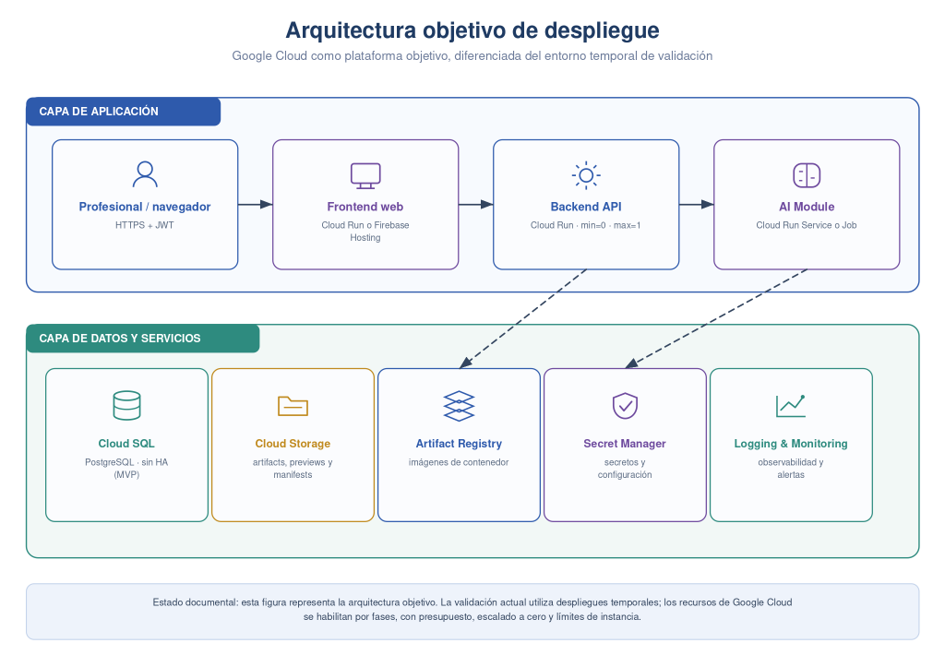
\includegraphics[width=0.92\textwidth]{images/architecture/fig_10_07_despliegue_google_cloud.png}
\caption{Arquitectura de despliegue validada en Google Cloud y servicios gestionados asociados. Fuente: elaboración propia.}
\label{fig:arch-despliegue-google-cloud}
\end{figure}

\section{Vista de escenarios (+1)}

Los escenarios articulan las cuatro vistas anteriores mediante casos de uso concretos. El escenario principal (autenticación, carga del estudio, ejecución multiplanar, persistencia, visualización y revisión profesional) recorre la vista de procesos (sección 10.4.1), se apoya en los componentes de la vista lógica y en la organización de la vista de desarrollo, y se ejecuta sobre la infraestructura de la vista física. Las historias de usuario del Capítulo 9 formalizan estos escenarios y permiten validar que la arquitectura satisface los requerimientos.
% CROSS_REFERENCE_NUMBERING_REVIEW_REQUIRED

\section{Diseño de interfaz: wireframes y decisiones de diseño}

Antes de implementar el frontend se elaboraron esquemas de interfaz que traducen las necesidades detectadas en el relevamiento a una disposición concreta de pantallas y componentes. Estos wireframes cumplen dos funciones dentro del proyecto: fijar el recorrido del profesional antes de escribir código y dejar explícita la relación entre cada zona de la interfaz y la necesidad que la origina. El diseño no persigue elaboración estética, sino legibilidad de resultados y disponibilidad permanente de la acción de revisión.

\subsection{Criterios de diseño derivados del user research}

El relevamiento estableció cuatro condiciones que la interfaz debe cumplir con independencia de su apariencia final.

\begin{itemize}
  \item La imagen original y la máscara superpuesta deben poder compararse sin cambiar de pantalla, y la superposición debe poder activarse y desactivarse (N-01).
  \item Toda estructura y toda medición deben ofrecer, en el mismo lugar donde se muestran, la posibilidad de aceptar, observar, corregir o descartar el resultado (N-02, N-05).
  \item Cada valor presentado debe indicar la estructura, el plano y el corte del que proviene, de modo que el profesional pueda verificar su origen (N-04, N-12).
  \item La ausencia de una secuencia, de un plano o de un resultado debe informarse de manera explícita, sin completar el espacio con información aproximada (N-11).
\end{itemize}

A estas condiciones se suma un criterio de eficiencia señalado en las entrevistas: el flujo no debe agregar tiempo innecesario respecto de la práctica actual (N-07). En consecuencia, el recorrido principal se diseñó con la menor cantidad posible de pantallas intermedias entre la carga del estudio y la visualización de resultados.

\subsection{Esquemas de las pantallas principales}

\begin{figure}[htbp]
\centering
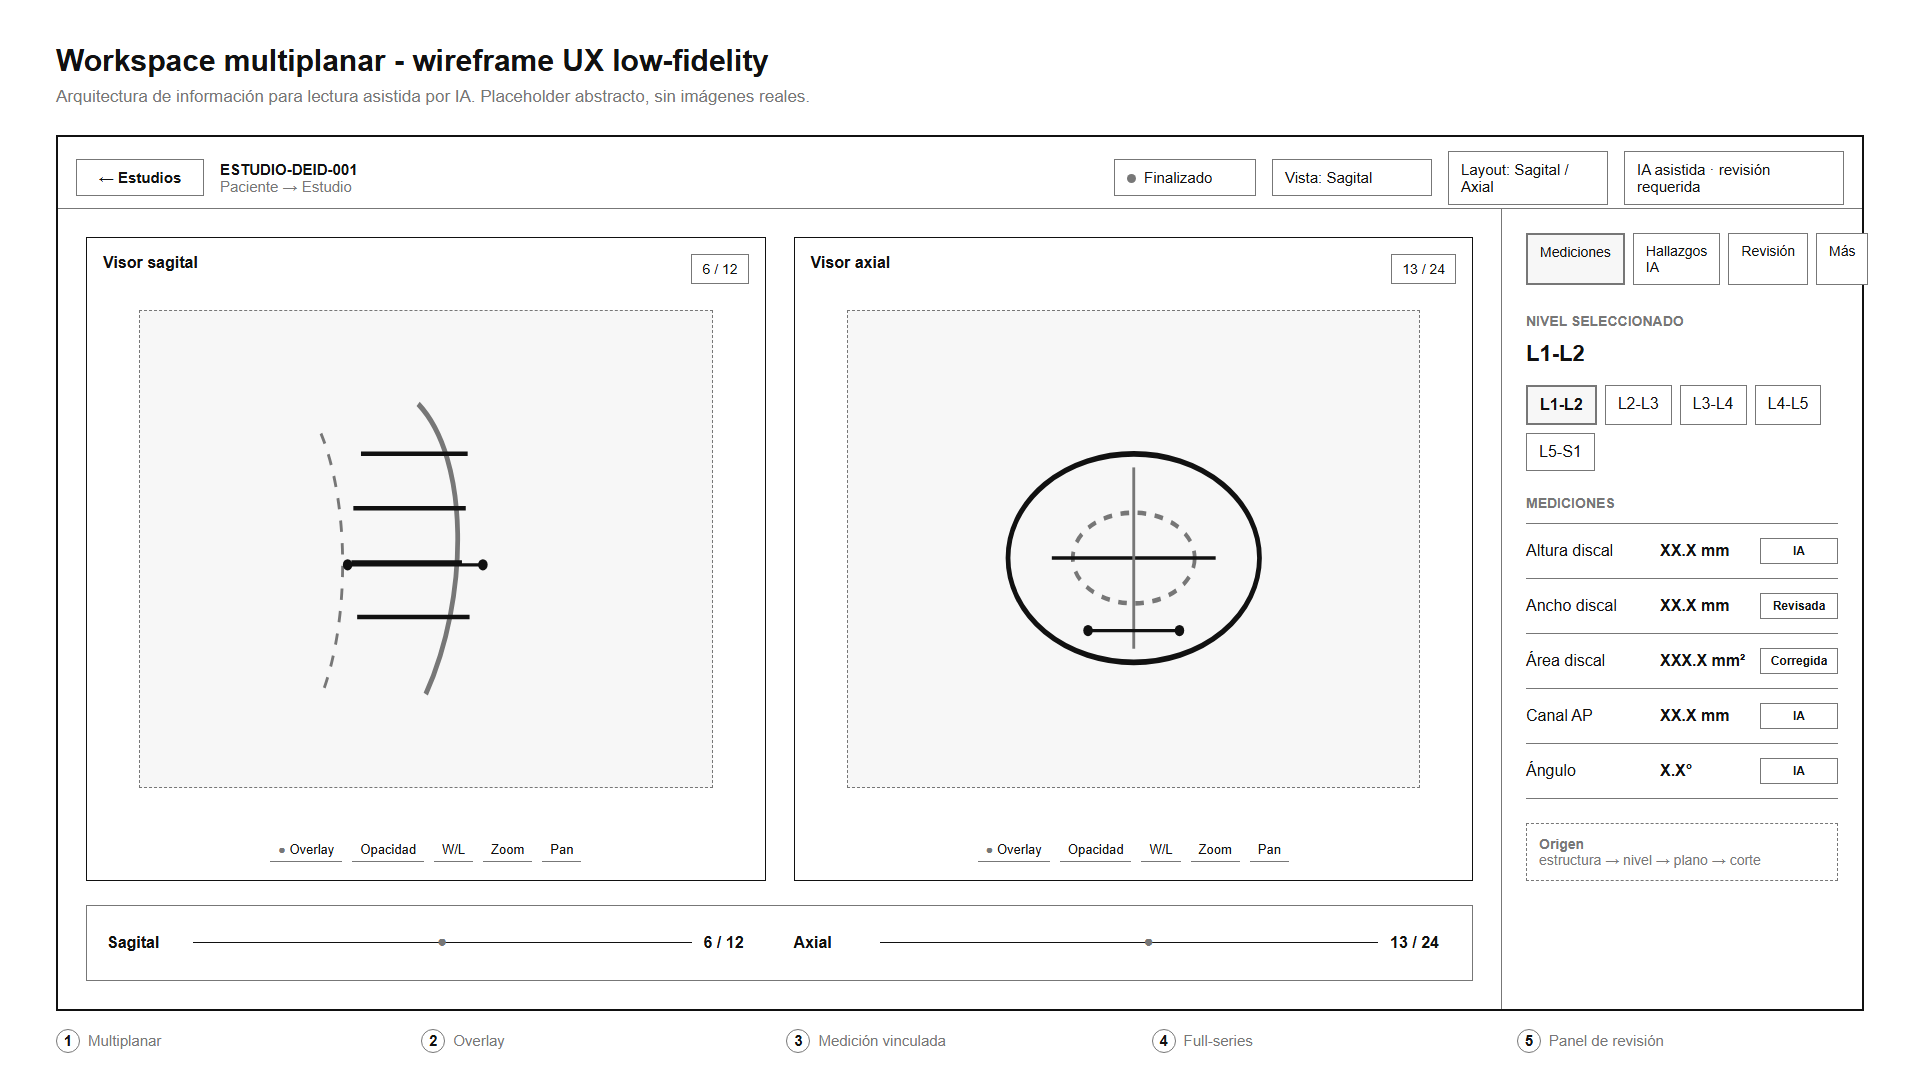
\includegraphics[width=\textwidth]{images/wireframes/fig_10_08_wireframe_workspace_multiplanar.png}
\caption{Wireframe de baja fidelidad del workspace multiplanar propuesto, incluyendo visualización sagital y axial, navegación full-series, superposición de resultados y panel de mediciones vinculadas al nivel anatómico. Fuente: elaboración propia.}
\label{fig:arch-wireframe-workspace-multiplanar}
\end{figure}

\begin{figure}[htbp]
\centering
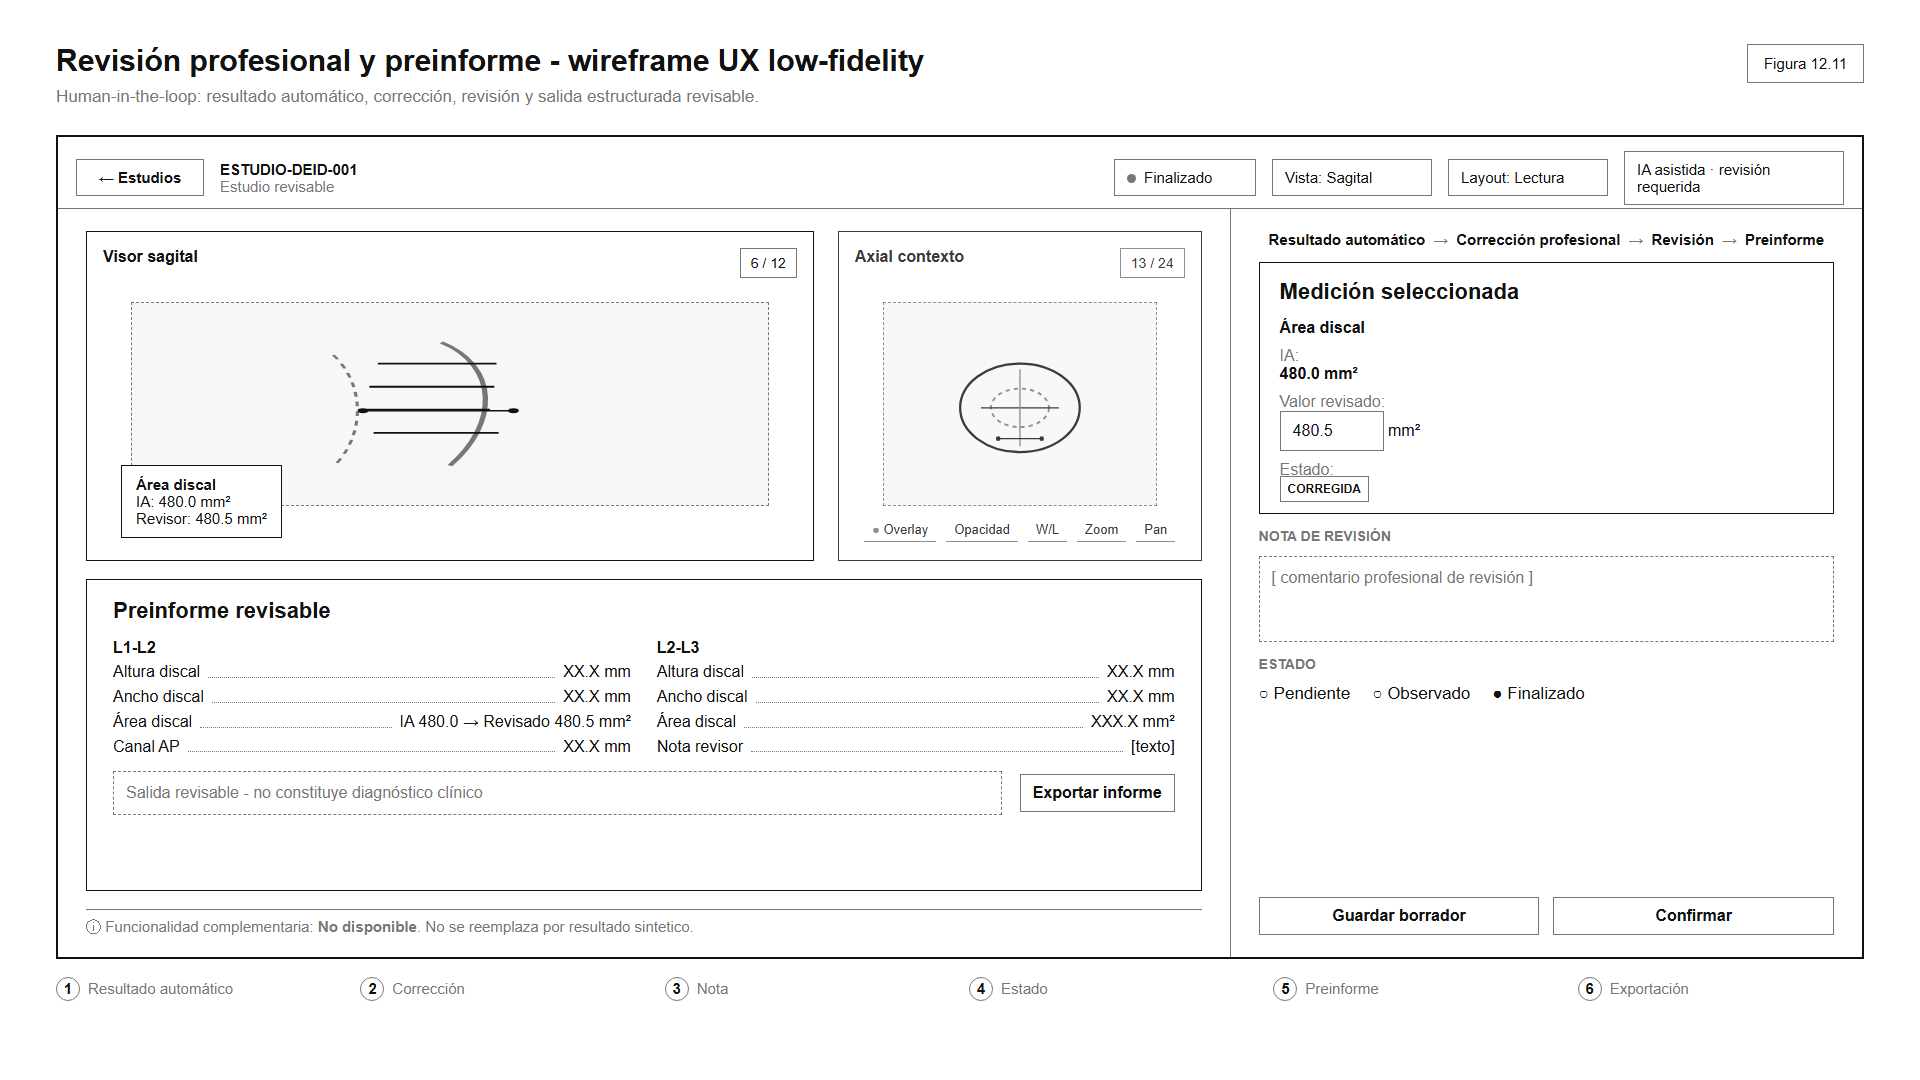
\includegraphics[width=\textwidth]{images/wireframes/fig_10_09_wireframe_revision_preinforme.png}
\caption{Wireframe de baja fidelidad del flujo de revisión profesional y preinforme, mostrando la trazabilidad entre el resultado automático, la corrección del profesional, el estado de revisión y la salida estructurada revisable. Fuente: elaboración propia.}
\label{fig:arch-wireframe-revision-preinforme}
\end{figure}

{\scriptsize
\setlength{\LTleft}{0pt}
\setlength{\LTright}{0pt}
\setlength{\tabcolsep}{2pt}
\renewcommand{\arraystretch}{1.18}
\begin{longtable}{>{\raggedright\arraybackslash}p{0.22\textwidth} >{\raggedright\arraybackslash}p{0.30\textwidth} >{\raggedright\arraybackslash}p{0.16\textwidth} >{\raggedright\arraybackslash}p{0.24\textwidth}}
\caption{Relación entre zonas de la interfaz, necesidades del relevamiento y requerimientos}\label{tab:arch-interfaz-trazabilidad}\\
\hline
\textbf{Zona de la interfaz} & \textbf{Función} & \textbf{Necesidad} & \textbf{Requerimiento} \\
\hline
\endfirsthead
\caption[]{Relación entre zonas de la interfaz, necesidades del relevamiento y requerimientos (continuación)}\\
\hline
\textbf{Zona de la interfaz} & \textbf{Función} & \textbf{Necesidad} & \textbf{Requerimiento} \\
\hline
\endhead
\hline
\endfoot
Worklist de estudios & Identificar casos disponibles, pendientes y revisados sin abrir cada uno. & N-07 & HU-02 \\
Alta de estudio y carga & Asociar el volumen a una referencia de sujeto seudonimizada e informar las series compatibles detectadas. & N-09, N-11 & HU-03, HU-04 \\
Visor con superposición conmutable & Comparar imagen original y máscara en el mismo encuadre. & N-01 & HU-06 \\
Selector de plano y navegación por cortes & Recorrer el volumen conservando la relación entre resultado y corte de origen. & N-03, N-12 & HU-07 \\
Panel de mediciones & Presentar cada valor junto con su estructura, plano y corte. & N-04 & HU-08 \\
Controles de revisión & Aceptar, observar, corregir o descartar cada resultado desde el punto en que se muestra. & N-02, N-05 & HU-09 \\
Preinforme editable & Reunir estructuras, mediciones, observaciones y estado de revisión en una salida modificable. & N-04, N-08 & HU-09 \\
Estados vacíos y degradados & Informar la ausencia de plano, secuencia o resultado sin completar la información faltante. & N-11 & HU-11 \\
Historial de corridas & Reabrir un estudio ya procesado sin repetir la inferencia. & N-08, N-10 & HU-10 \\
\hline
\end{longtable}
}

\subsection{Decisiones de diseño y alternativas descartadas}

Tres decisiones merecen registro porque condicionaron la implementación posterior.

La primera es la disposición del panel de revisión junto al visor y no en una pantalla posterior. El relevamiento indicó que la corrección forma parte de la lectura y no de una etapa separada, de modo que separar ambas acciones habría agregado un paso sin valor clínico.

La segunda es la decisión de no mostrar probabilidades ni puntajes de confianza numéricos al usuario final. Las entrevistas señalaron que un valor de confianza sin validación clínica puede inducir una interpretación indebida, por lo que la interfaz comunica el estado del resultado en términos operativos y no probabilísticos.

La tercera es la presentación del plano axial como vista complementaria y no como pestaña equivalente al sagital. Esta decisión refleja el alcance real del prototipo, en el que la base anatómica y la mayor parte de la validación técnica se apoyan en el plano sagital, y evita sugerir una paridad de madurez entre ambos módulos.
